\documentclass[11pt,a4paper]{article}
\usepackage[margin=1in]{geometry}
\usepackage{booktabs,graphicx,float,longtable,hyperref,xcolor}
\usepackage[default]{sourcesanspro}
\hypersetup{colorlinks=true,linkcolor=blue,urlcolor=blue}
\title{AG News Topic Classification\\\large TF--IDF Baseline and DistilBERT Data-Efficiency Study}
\author{Mohammad Torabi \\ 404422041}
\date{Course: Data Mining \\ Instructor: Dr. Hadi Farahani \\ August 2026}
\begin{document}
\maketitle

\begin{abstract}
In this project, I classify AG News articles into four topics with a TF--IDF Logistic Regression baseline and a fine-tuned DistilBERT model. My original contribution is a data-efficiency experiment: I train the same DistilBERT setup with 10\%, 25\%, and 100\% of a fixed 3,000-article training subset. On the fixed 1,000-article test subset, the full DistilBERT run obtains 0.899 accuracy and 0.899 macro-F1. It is better than the TF--IDF baseline by 0.045 macro-F1, although the small one-epoch experiment should not be considered a final benchmark.
\end{abstract}

\section{Problem, Data, and Contribution}
The task is four-class English news classification: World, Sports, Business, and Sci/Tech. I used a shuffled subset of 3,000 training articles and 1,000 test articles with seed 42. The classes are balanced in the original dataset, and the selected split also contains all four topics. Figure~\ref{fig:balance} and Table~\ref{tab:balance} show the class distribution from the exploratory notebook.

My question is simple: how much labelled data is needed before fine-tuned DistilBERT becomes useful compared with a classical sparse baseline? I expect that more examples will generally help, but a small run can have variation because it uses only one epoch.

\begin{table}[H]\centering
\caption{AG News class distribution in the original dataset.}\label{tab:balance}
\begin{tabular}{lrr}\toprule
Class & Training articles & Test articles \\\midrule
World & 30,000 & 1,900 \\ Sports & 30,000 & 1,900 \\
Business & 30,000 & 1,900 \\ Sci/Tech & 30,000 & 1,900 \\\midrule
Total & 120,000 & 7,600 \\\bottomrule
\end{tabular}
\end{table}
\begin{figure}[H]\centering
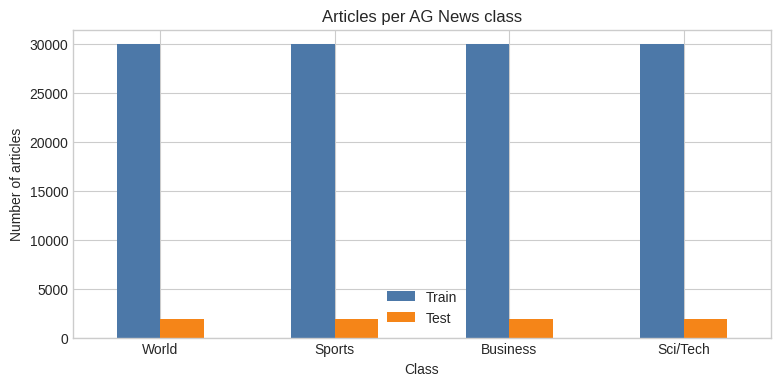
\includegraphics[width=.82\linewidth]{figures/class_balance.png}
\caption{The four AG News labels are balanced.}\label{fig:balance}
\end{figure}

Articles are short in this dataset. The class medians in the exploratory analysis are between 36 and 39 words, so a maximum length of 128 tokens is a reasonable practical choice. Figure~\ref{fig:lengths} also shows that there is a smaller long-article tail.
\begin{figure}[H]\centering
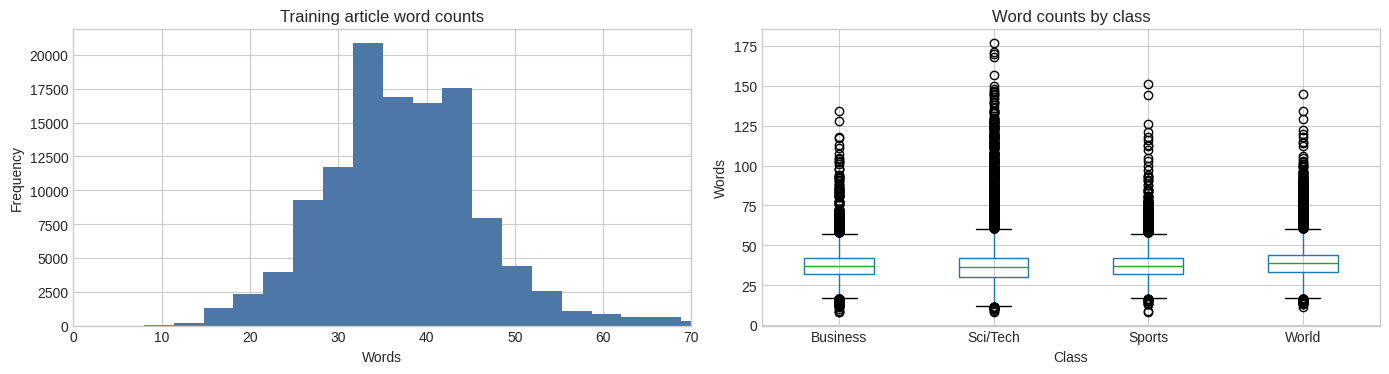
\includegraphics[width=\linewidth]{figures/article_lengths.png}
\caption{Article-length distribution in the selected training data.}\label{fig:lengths}
\end{figure}

\section{Method and Experimental Setup}
The baseline uses TF--IDF unigram and bigram features, at most 20,000 features, \texttt{min\_df=2}, and Logistic Regression with 200 maximum iterations. The neural model is \texttt{distilbert-base-uncased}. For every DistilBERT condition, I use maximum length 128, AdamW with learning rate $5\times10^{-5}$, batch size 8, one epoch, and seed 42.

The baseline uses all 3,000 selected training rows. DistilBERT is trained three times with 300, 750, and 3,000 rows. All conditions are evaluated on the same 1,000 selected test rows. I report accuracy and macro-F1 because the classes are balanced; macro-F1 also checks that a model does not improve only one class.

\section{Results and Analysis}
Table~\ref{tab:results} contains the saved experiment results. The 100\% DistilBERT model is best: 0.899 accuracy and 0.899 macro-F1. This is 0.044 accuracy points and 0.045 macro-F1 points above TF--IDF Logistic Regression. The 10\% model already reaches 0.870 macro-F1, but the 25\% model falls to 0.855. I do not interpret this as evidence that more data is harmful. With one epoch and a small subset, optimization randomness and sample composition can affect the result. The main observation is that the full-data condition is clearly strongest among my runs.

\begin{table}[H]\centering
\caption{Saved test-set results on the same 1,000 selected articles.}\label{tab:results}
\begin{tabular}{lrr}\toprule
Run & Accuracy & Macro-F1 \\\midrule
TF--IDF + Logistic Regression & 0.855 & 0.854 \\
DistilBERT, 10\% (300 rows) & 0.870 & 0.870 \\
DistilBERT, 25\% (750 rows) & 0.857 & 0.855 \\
DistilBERT, 100\% (3,000 rows) & \textbf{0.899} & \textbf{0.899} \\\bottomrule
\end{tabular}
\end{table}
\begin{figure}[H]\centering
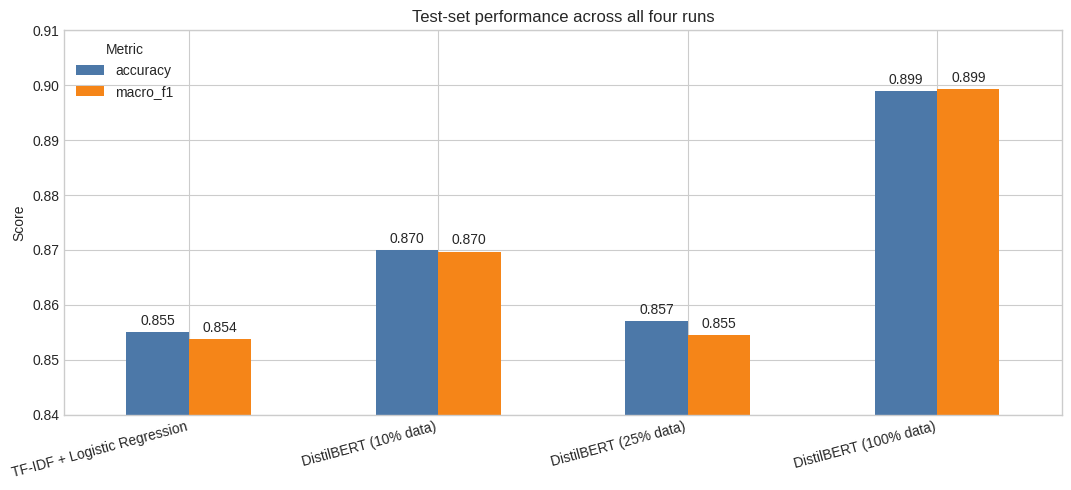
\includegraphics[width=\linewidth]{figures/model_comparison.png}
\caption{Accuracy and macro-F1 for the baseline and data-efficiency conditions.}\label{fig:comparison}
\end{figure}
\begin{figure}[H]\centering
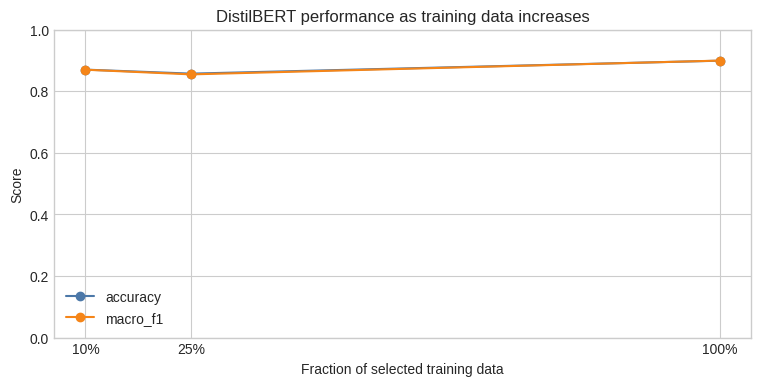
\includegraphics[width=.82\linewidth]{figures/data_efficiency.png}
\caption{DistilBERT performance as more selected training data is used.}\label{fig:efficiency}
\end{figure}

\section{Prediction Demo and Limitations}
The notebook demo loads the saved TF--IDF pipeline and the three saved DistilBERT checkpoints. The models agree on six hand-written news-style examples. This is useful for checking the saved artifacts, but it is not a strong error analysis because the examples are easy and not sampled from real mistakes.

Important limitations are the one-epoch budget, 3,000/1,000 subset, and missing saved per-class predictions. A stronger next experiment would train for several seeds, use the full test split, save confusion matrices and per-class F1, and inspect genuine errors. The reported values are real saved outputs, but their scope is only this CPU-sized experiment.

\section{Discussion and Observation}
\subsection*{Convolution and self-attention}
A one-dimensional convolution is good at detecting nearby patterns, for example a short phrase such as ``not expected to play.'' It has a local receptive field and a useful locality bias. Self-attention can connect distant words directly and can decide which words are important for each other. For a sentence where a late phrase changes the meaning of an earlier sports result, I expect attention to use the long-distance relation more easily than a shallow convolution. On the other hand, attention does not automatically have the same local preference as convolution.

\subsection*{A hybrid design}
I could place a small convolution before self-attention to produce local phrase features, then let attention combine them across the article. Another choice is to add convolution inside a Transformer feed-forward part. In both cases, convolution contributes local word-order patterns and attention contributes global context. I would test this only with a controlled comparison, because it also increases the number of parameters.

\section{Reproducibility}
From the project directory, run \path{python scripts/train.py}. The script writes \path{outputs/results.csv}, the TF--IDF pipeline, and the three DistilBERT checkpoints. The report figures are static exports from the notebooks, so the report can compile without downloading models again.
\end{document}
